\chapter{Methodology}

\section{Research Methodology and Project Approach}

The project uses a design oriented, prototype based research methodology. It develops and evaluates a blockchain based, community assisted, privacy preserving reporting system for local governance. The primary focus is on systematic system design, functional prototyping, and controlled experimental evaluation. It does not focus on large-scale real-world deployment. The methodology follows a structured, step by step system development lifecycle. The workflow begins with requirement analysis and conceptual system design. This is followed by implementation of a permissioned blockchain, smart contracts, off chain services and also AI assisted modules. The system is evaluated and incrementally integrated using functionality metrics and predefined performance and this phased approach ensures traceability between objectives, design decisions, implementation steps, and also evaluation outcomes. Figure~\ref{fig:implementation-methodology} illustrates the overall implementation methodology.

\begin{figure}[h!]
    \centering
    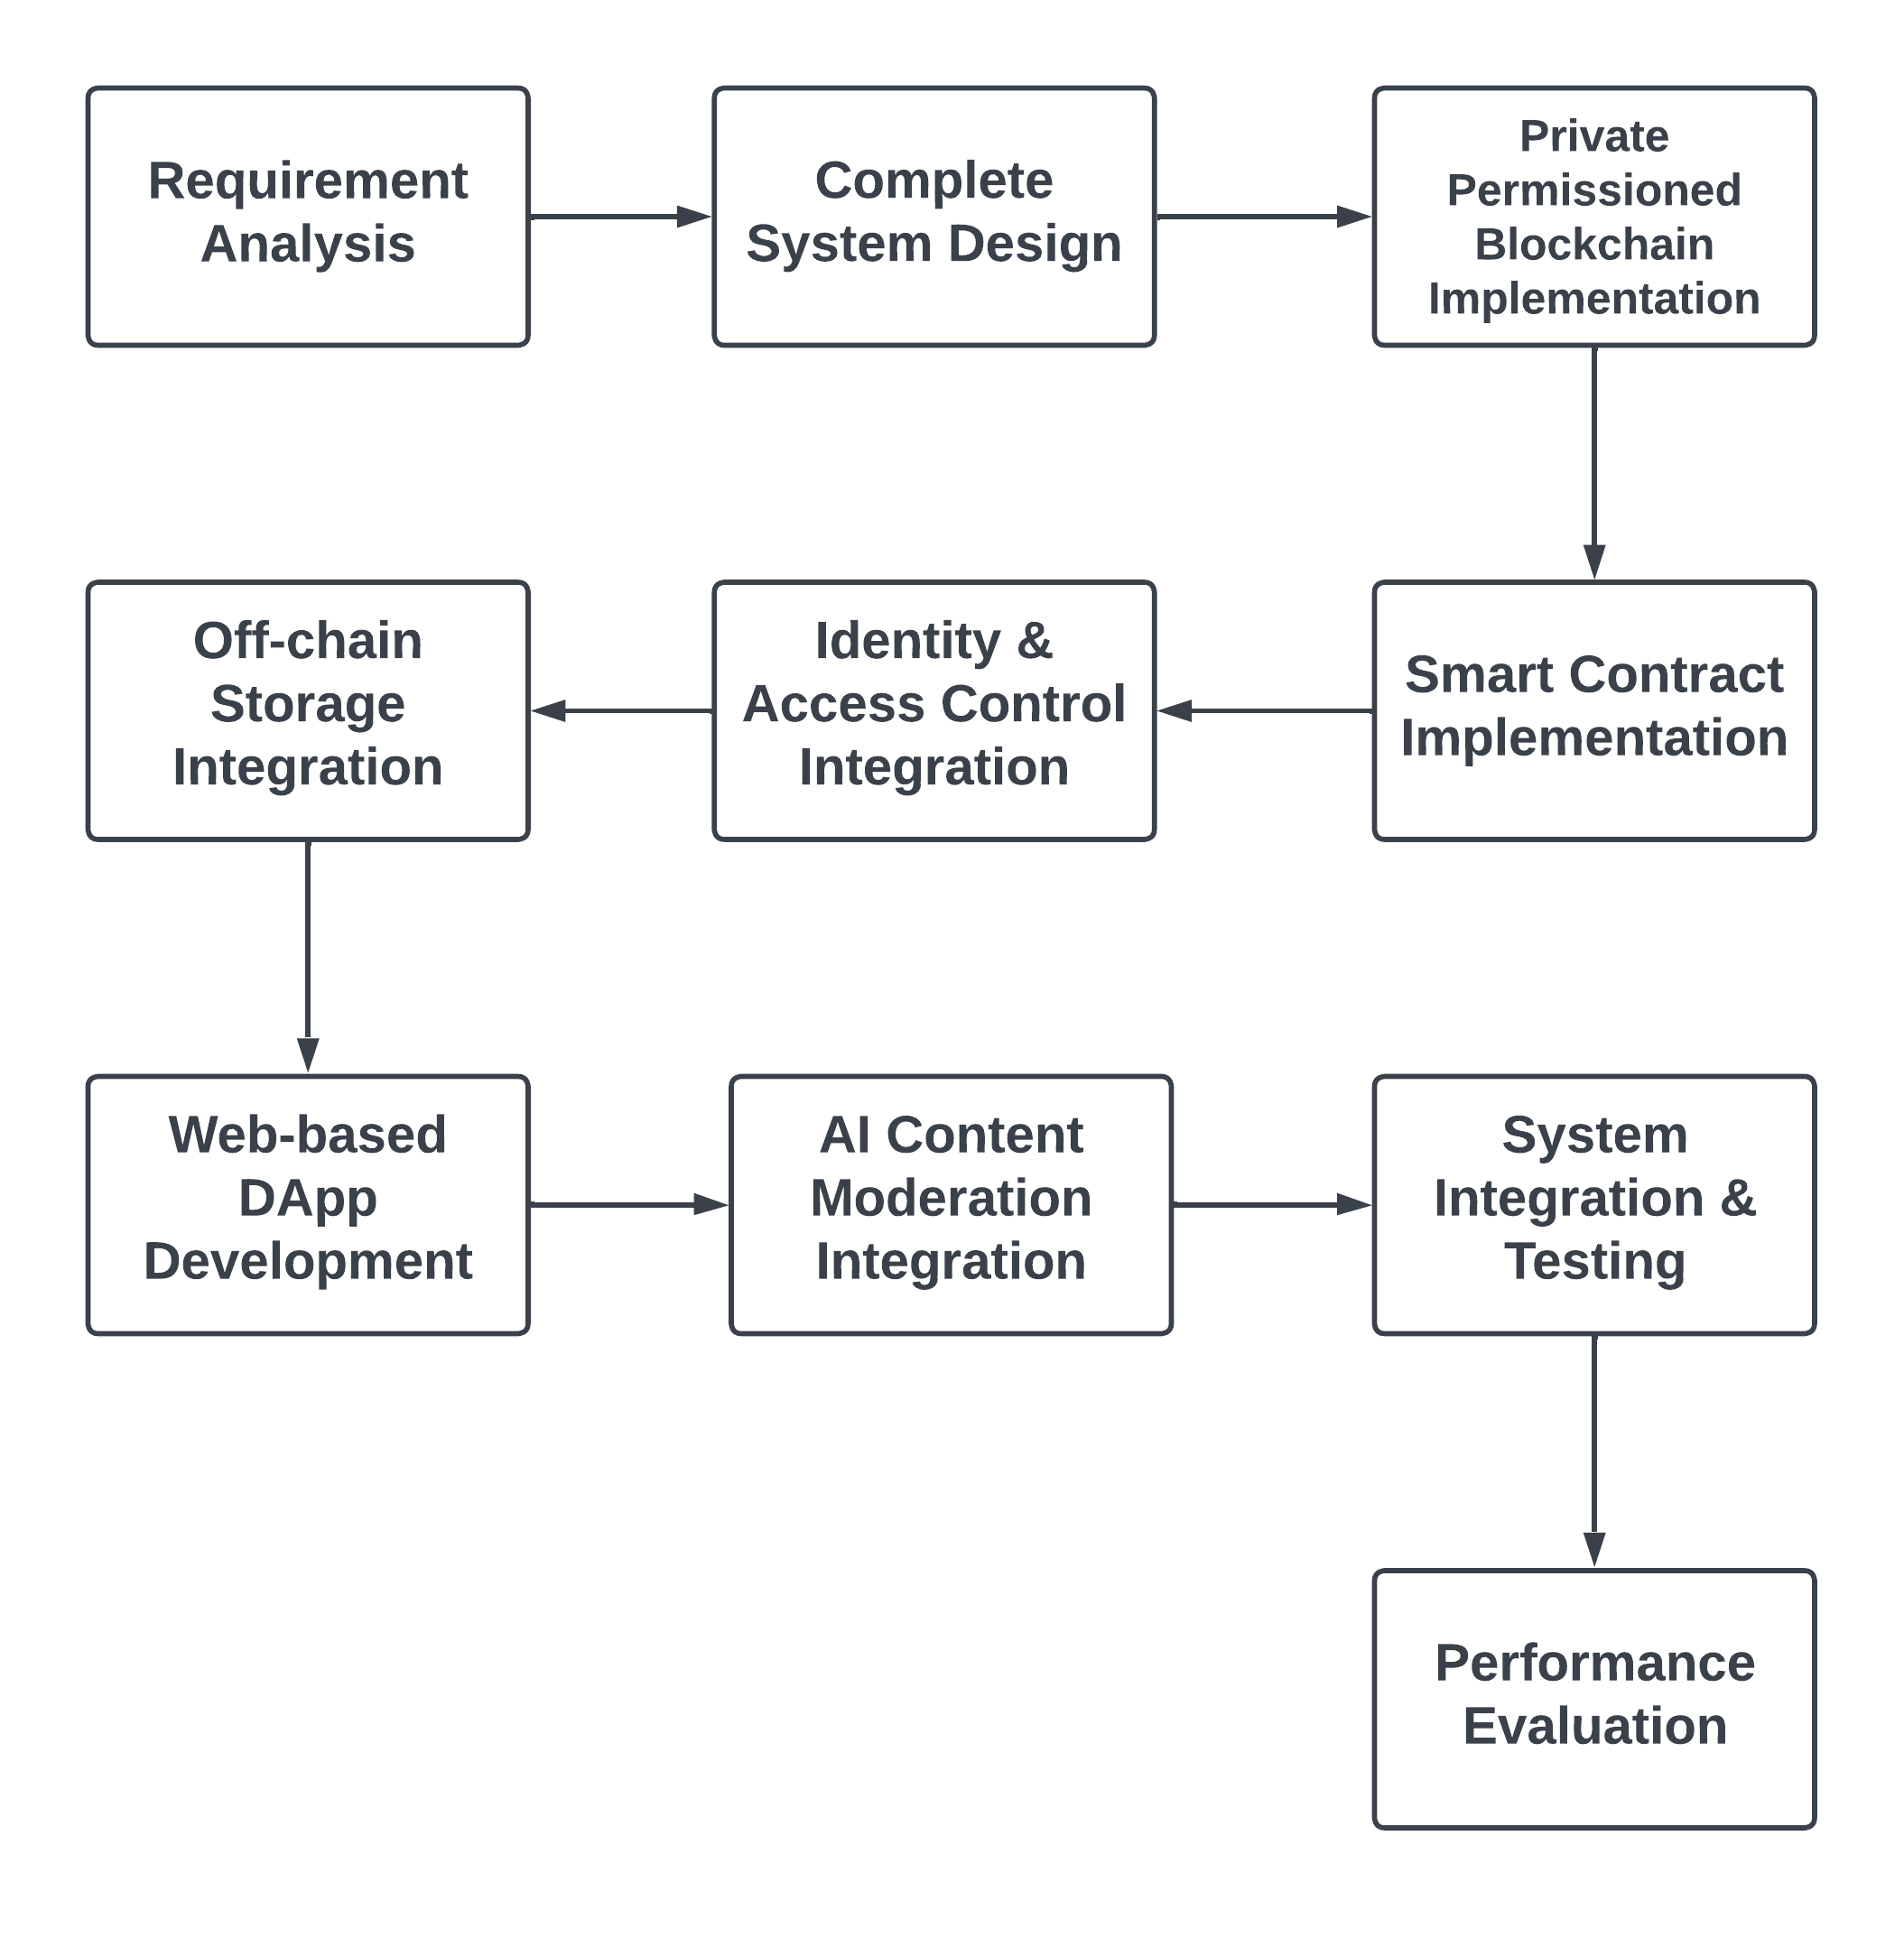
\includegraphics[width=0.95\textwidth]{figures/implementation-methodology.png}
    \caption{Step-by-Step Implementation Methodology for the Proposed System}
    \label{fig:implementation-methodology}
\end{figure}

\section{Requirement Analysis}

Requirement analysis phase identifies functional and non-functional requirements based on project objectives and literature review insights. Citizen issue reporting, community voting, opinion polling, issue tracking, and authority side resolution updates are Functional requirements. Transparency, data integrity, privacy preservation, scalability, and usability are non functional requirements. 

This phase is designed using literature driven requirement extraction approach. Existing blockchain based governance systems and digital reporting platforms are analyzed to get an idea. Use case scenarios for government officials and citizens are defined to guide subsequent system design decisions.

\section{Complete System Design}

A comprehensive system design phase is carried out based on identified requirements. The design defines overall architecture, data flows and access control techniques. The system uses a layered architecture. It separates concerns between user interaction, identity management, logics in application, blockchain enforcement, off chain storage, AI services. The architectural design gives modularity for independent development and testing of components. The system design is developed using high level architectural diagrams and workflow. Figure~\ref{fig:architectural-diagram.png} illustrates the high level architecture of the system.

\begin{figure}[h!]
    \centering
    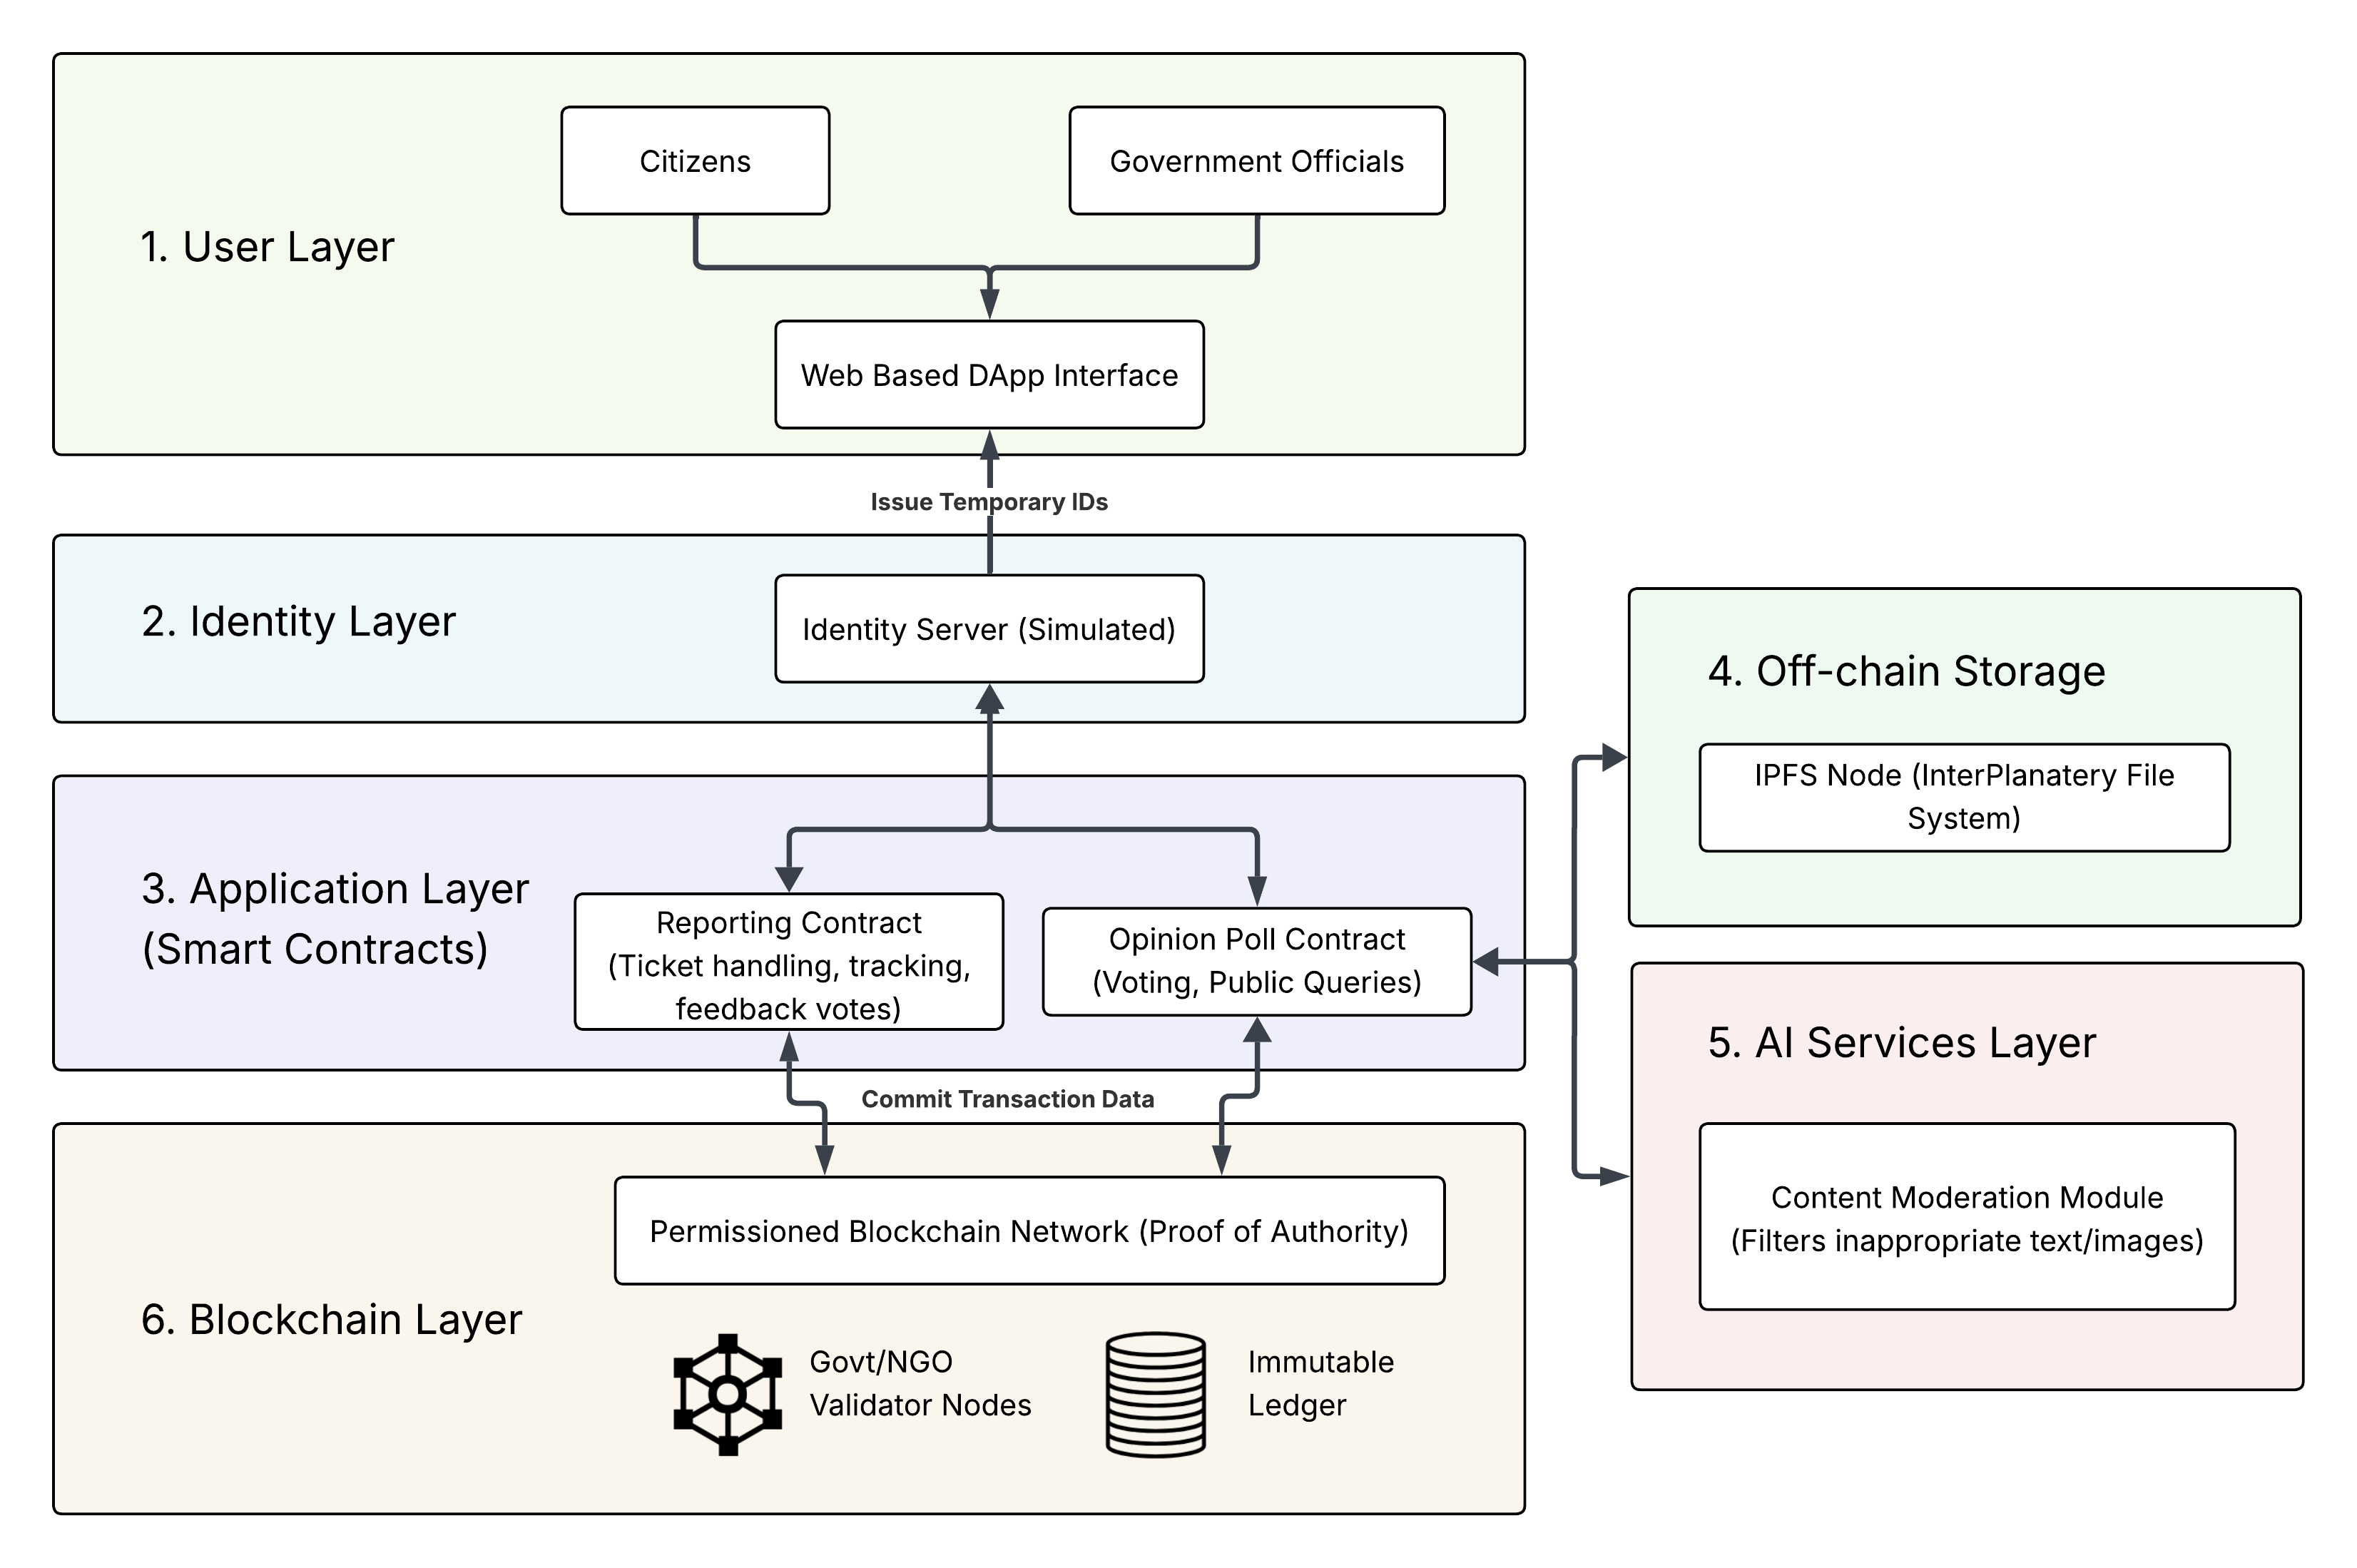
\includegraphics[width=0.95\textwidth]{figures/architectural-diagram.png}
    \caption{High-Level Architectural Diagram of the Proposed System}
    \label{fig:architectural-diagram.png}
\end{figure}

\section{Private Permissioned Blockchain Implementation}

A private permissioned blockchain network is implemented to ensure controlled participation, data integrity and also immutability of submitted records. The blockchain operates under a \ac{PoA} consensus mechanism. Validator nodes are assumed to be operated by trusted government or any other organizations. 

The permissioned setup reduces transaction latency and energy consumption compared to public blockchains. The blockchain records report metadata, state transitions, voting, and hashes of off chain content.

\section{Smart Contract Implementation}

Report submission, ticket creation, community voting, issue status updates, resolution confirmation, closure, and public opinion polling are core reporting workflows of this system. Smart contracts are designed and implemented to automate the above mentioned core reporting workflows. 

The Contracts consider about predefined business logic and access control rules to ensure only authorized users can perform specific actions. Smart contracts are developed using Solidity. permissioned blockchain network is used to deploy Contracts. Contract functionality is tested in a local development environment to validate state transitions and data consistency.

\section{Identity and Access Control Integration}

A simulated identity and access control mechanism is integrated into the system to preserve user anonymity while enabling accountability. The platform is accessed by the users via pseudonym identifiers distributed by the simulated identity server. Role-Based Access Control differentiates between citizens and government authorities. This is the embodiment of principles of Decoupling Identity without building the full concept of SSI Systems. Verification of identity and access is implemented through application logic and Smart Contract validation.

\section{Off-chain Storage Integration}

Multimedia content related to reports cannot be recorded on-chain due to limitations of blocks in the blockchain. Therefore, IPFS is used to store multimedia content as a decentralized, off-chain storage. When a user submits a report with multimedia content, the media is uploaded to IPFS and the cryptographic hash related to that media is recorded on-chain via smart contracts. This method ensures data integrity and verifiability of the report. Also it minimizes the on-chain storage overhead and improves the system scalability.

% Due to the storage limitations of blockchain systems, multimedia content such as images and videos associated with reports is stored off-chain. The \ac{IPFS} is used as the decentralized storage solution.


% When a user submits multimedia content, the data is uploaded to IPFS, and the resulting cryptographic hash is recorded on the blockchain via smart contracts. This approach ensures data integrity and verifiability while minimizing on-chain storage overhead and improving system scalability.

\section{Web-based Decentralized Application Development}

A \ac{DApp} is developed to provide user interfaces for citizens and government officials. By using \ac{DApp} users can submit reports, participate in voting, view issue statuses, and interact with the blockchain network. The frontend is implemented using modern web development frameworks such as Vite, NextJS. Web3 libraries are used to handle blockchain interaction. The \ac{DApp} communicates with smart contracts deployed on the permissioned blockchain and integrates with IPFS and AI module which are stored off-chain.

% \section{Trustworthiness Mechanism Integration}

% To improve the reliability of community participation, a trustworthiness evaluation mechanism is integrated into the system. Trust scores are computed based on user behavior, including historical report validity and peer-validation outcomes.

% The trustworthiness evaluation is performed off-chain using lightweight analytical or AI-assisted models, and the resulting scores influence voting weights and report prioritization. This mechanism enhances data quality while preserving user anonymity and preventing reliance on personal identity data.

\section{AI-Based Content Moderation Integration}

The AI-based content moderation module is used to detect and filter inappropriate textual and visual content in user-submitted reports. The moderation process is executed off-chain prior to blockchain submission. In this component, existing pretrained AI models or external content moderation APIs are used.

\section{System Integration and Testing}

To implement the proposed blockchain-based community-assisted reporting system successfully, we need a structured testing procedure. Because blockchain-based records are immutable, bugs introduced in later stages are difficult to correct. Therefore, we will use a testing methodology with early validation and progressive integration throughout the development period. 

The project team will conduct all testing activities within a controlled environment. Each subsystem is tested by the team member responsible for its design and implementation. It is followed by joint integration testing to ensure all modules interact correctly. 

\subsection{Testing Responsibilities and Approach}

Testing responsibilities are distributed according to system functionality. The project team performs the following testing tasks collectively. 
\begin{enumerate}[i]
    \item Blockchain and smart contract testing. (transaction execution,
    access control, workflow validation)
    \item Web interface testing (user interactions, data submission, status visualization)
    \item AI module testing (appropriate filtering of textual and visual
    content)
    \item Integration testing (data flow across the blockchain, AI services,
    off-chain storage, and user interface layers)
\end{enumerate}

\subsection{Data Acquisition and Test Data Generation}

Because the system is evaluated within a controlled experimental environment, testing relies on a combination of synthetic data and publicly available datasets. The different categories of test data used in the project and their purposes are summarized in Table~\ref{tab:data-acquisition}.

\begin{table}[h!]
\centering
\small
\renewcommand{\arraystretch}{1.4}
\caption{Test Data Sources and Usage}
\label{tab:data-acquisition}
\begin{tabular}{|p{4cm}|p{4cm}|p{5cm}|}
\hline
\textbf{Data Type} & \textbf{Data Source} & \textbf{Purpose in Testing} \\ \hline

Synthetic Reporting Data &
Programmatically generated using scripts and mock user profiles &
Simulation of citizen reports, voting actions, issue resolution events, and validation of blockchain workflows and smart contract execution \\ \hline

Textual Content Samples &
Publicly available moderation datasets and manually curated samples &
Evaluation of AI-based text moderation for detecting inappropriate, irrelevant, or malicious textual content \\ \hline

Visual Evidence Samples &
Public urban infrastructure datasets (e.g., potholes, garbage, road damage images) &
Testing image-based content moderation, off-chain storage via IPFS, and hash integrity verification \\ \hline

\end{tabular}
\end{table}


The use of synthetic and publicly available datasets ensures ethical compliance,
repeatability, and controlled experimentation.

\subsection{Subsystem-Level Testing}

According to the Table \ref{tab:testing-plan}, all major subsystems are tested independently before full system integration.

\begin{table}[h!]
\centering
\small
\renewcommand{\arraystretch}{1.4}
\caption{Subsystems and Planned Testing Activities}
\label{tab:testing-plan}
\begin{tabular}{|p{5.5cm}|p{7.5cm}|}
\hline
\textbf{Subsystem} & \textbf{Testing Method} \\ \hline

Permissioned Blockchain Network &
Functional testing of transaction validation, block creation, and validator authorization under PoA consensus \\ \hline

Smart Contract Logic &
Unit testing of report creation, feedback voting, status transitions, issue closure, and opinion polling workflows \\ \hline

User Interface Module &
Functional and usability testing of report submission, issue tracking, feedback voting, and polling interactions \\ \hline

AI-Based Content Moderation &
Validation of text and image filtering accuracy using synthetic and public datasets \\ \hline

Off-Chain Storage Module &
Testing of file uploads, hash generation, and integrity verification between IPFS and blockchain \\ \hline

End-to-End System Integration &
Scenario-based testing of complete workflows from report submission to issue closure  \\ \hline

\end{tabular}
\end{table}

\subsection{System Integration Testing}

After successful subsystem testing, end-to-end integration testing is performed.
Complete reporting scenarios are simulated, starting from report submission and
content moderation to blockchain recording, community feedback voting, issue
resolution updates, and final closure.

In the integration test, we mainly focus on  consistent data flow, correct state
synchronization, and reliable interaction between all system components.

\section{Performance Evaluation}

% The performance evaluation assesses the operational feasibility of the proposed
% system within a controlled experimental environment. The objective is not to
% benchmark production-level performance but to demonstrate that the architecture
% can reliably support community-assisted reporting workflows.
The performance evaluation evaluates the operational feasibility of the proposed system within a controlled experimental environment. The objective is to demonstrate that the architecture can reliably support community-assisted reporting workflows. It will not benchmark production-level performance. 

\subsection{Evaluation Environment}

The evaluation environment consists of a private, Ethereum-compatible blockchain network. This network is configured with a \ac{PoA} consensus mechanism. We will test the system using simulated users and synthetic workloads generated by the project team.

\subsection{Evaluation Metrics}

The performance and reliability of the proposed system are evaluated using the evaluation metrics stated in the Table~\ref{tab:evaluation-metrics}.

\begin{table}[h!]
\centering
\small
\renewcommand{\arraystretch}{1.4}
\caption{System Evaluation Metrics}
\label{tab:evaluation-metrics}
\begin{tabular}{|p{4cm}|p{10cm}|}
\hline
\textbf{Metric} & \textbf{Description} \\ \hline

Transaction Latency &
Time required for report submissions, voting actions, and status updates to be
confirmed on the blockchain \\ \hline

Transaction Throughput &
Number of transactions processed per unit time during simulated reporting and
community voting activity  \\ \hline

Smart Contract Execution Reliability &
Consistency and correctness of smart contract execution during repeated workflow
operations \\ \hline

AI Moderation Response Time &
Time taken for text-based and image-based content moderation decisions to be
returned and integrated into the workflow  \\ \hline

Off-Chain Storage Performance &
Time required to upload and retrieve multimedia evidence from off-chain storage  \\ \hline

\end{tabular}
\end{table}


\subsection{Testing Procedure}

Performance testing is conducted by gradually increasing the number of simulated reports and feedback votes submitted to the system. All transaction logs and execution results are recorded. Those records will then be analyzed to observe latency trends, system stability, and failure conditions.

\subsection{Limitations}

The performance evaluation is limited to prototype deployment using simulated
data in a controlled environment. Real-world network conditions, large-scale user
adoption, and institutional deployment constraints are outside the scope of this
project. 
